% Chapter Template

\chapter{State of the art} % Main chapter title

\label{Chapter2} % For referencing this chapter elsewhere, use \ref{Chapter2}

%----------------------------------------------------------------------------------------
%	SECTION 1
%----------------------------------------------------------------------------------------

\section{A taxonomy of the existing task scheduler paradigms}

The existing distributed system architectures --and also the existing distributed satellite systems-- can be classified according to the degree of centralization, from completely hierarchical systems to fully independent nodes. The research in the distributed algorithms field can also be divided into centralized and non-centralized paradigms, although it is not limited to that. However, completely new problems appear in the distributed systems, such as synchronization, leader election or data consistency,  and every different problem opens new approaches and new paradigms.

In particular, into the field of task scheduling, many approaches have been taken. There are plenty of scheduling policies and algorithms that could be compared with the Local-Global, from high-complexity fully-centralized algorithms that may be solved using dynamic or constraint programming (mainly for grid-computing or High Performance Computing, as in \cite{anderson2005high,ramamritham1984dynamic,yu2005taxonomy}), to low-computational decentralized schedulers \citep{1310996,zhu2007tasks}.

In the last years, distributed task scheduler research has mainly worked over three different paradigms, although not all of them have been applied to the distributed satellite systems context:

\begin{itemize}
\item \textbf{Negotiation or consensus} policies, in which nodes in the system \emph{agree} the final schedule, such as the distributable scheduling proposed in \cite{anderson2007consensus} for a distributed real-time system with hard end-to-end time constrains in the activities executed in parallel threads or the consensus protocol for balancing the burden of distributed applications execution in IoT contexts presented in \cite{colistra2014problem} 

Other examples of this type of distributed consensus-based schedulers are the algorithm presented in \cite{pilloni2012decentralized} --which is based on an iterative and asynchronous local optimization of the tasks allocations between neighbour nodes-- and the price-based\footnote{In a price-based consensus algorithm each node in the system calculates a bid depending on their knowledge and state, and the lowest value is chosen as the agreed value.} approach for balancing energy consumption among nodes in WSNs of \cite{Edalat09}.

Two very interesting approaches can also be found in \cite{choi2009consensus} and in \cite{bonnet2008coordination}. The contexts are very similar to the ABS satellite constellation. In the first policy, a combination of consensus and auction-based decision-making is used to coordinate a fleet of autonomous vehicles (UAVs) with two decentralized algorithms. The second paper describes a communication-constrained task allocator in the same context of that of ABS project: a satellite constellation.

\item \textbf{Centralized} optimized schedulers --where the degree of centralization can vary--, such as the solution presented in \cite{pilloni2011deployment}, in which a \emph{Coordinator} that possesses all the intelligence of the network is in charge of planning the job distribution in a WSN or the multiserver-oriented algorithm of \cite{servers} where a central job scheduler measures the server idle-time measurements to balance the servers load.

\item The more recent \textbf{bio-inspired} approaches --which take profit from observing and imitating the behaviour of the distributed systems present in the nature--, such as the adaptation of the stigmergy used by ants to stablish an optimal path of \cite{Stigmergy} or the resources balancing technique extracted from the one observed in ant colonies \citep{antcollonies}. These techniques are the least explored and applied for distributed satellite systems.
\end{itemize}

%OJOOOOOOOOOOOOOOOOOOOOOOOOOOOOOOOOOOOOOOOOOOOOOOOOOOOOOOOO
%--it can be done \emph{offline} as well as \emph{online}--
%OJOOOOOOOOOOOOOOOOOOOOOOOOOOOOOOOOOOOOOOOOOOOOOOOOOOOOOOOO

%Of these three categories, the one which almost unexplored is the third one: the research on it is almost only theoretical and only simple and descriptive approaches have been published. Usually they propose a procedure that imitates an observed behaviour on ant colonies or other such distributed \emph{nature} systems. For instance, an adaptation of the stigmergy used by ants to stablish an optimal path is presented in \cite{Stigmergy} and a resources balancing technique extracted from the one observed in ant colonies is described in \cite{antcollonies}. Although these are very interesting approaches, they are still not quite practical for the comparison that has been carried in this work.

On the other hand, the Local-Global policy could be described as a hybrid distributed algorithm\footnote{Local-Global policy combines the hierarchy of centralized approaches in the \emph{Global} entity while sharing the computational load among all the nodes for a fully-distributed resolution of the scheduling problem.}. Among all the algorithms presented a candidate for the comparison with the Local-Global must be chosen. To do so, some of the most interesting approaches that have been found, and what are the reasons for having chosen a particular one, will be briefly described in the next section.

%----------------------------------------------------------------------------------------
%	SECTION 2
%----------------------------------------------------------------------------------------

\section{Comparison: algorithms chosen to benchmark the Local-Global}

Having explored the paradigms that are being investigated in the distributed task scheduler field, a state-of-the-art algorithm must be found out for the comparison with the Local-Global policy: it should be designed for (or applicable in) similar contexts and resource requirements.

As it has been already stated, the research in the field of distributed satellite systems task schedulers is still in its first steps. Moreover, the computational capabilities of nano-satellites have been traditionally very low to consider a fully-autonomous system-wide distributed task scheduler running on every node. Furthermore, distributed satellite missions are still unfeasible due to the lack of accurate Inter-Satellite Links (ISL)\footnote{ISLs are stand-alone communication links among two or more satellites, not depending on the ground station.} for huge constellations of satellites. For this reason, the research on the distributed satellite system schedulers cannot be applied to real environments yet.

Relevant papers presenting distributed task schedulers suitable for similar contexts to ABS are only a few, as many times some characteristics of the presented system are too different to compare this policy with. There are policies for nearly infinite bandwidth communication among nodes, multi-processor scheduling algorithms, distributed task allocators for nodes with high computational capabilities...

The context in which the Local-Global policy is meant to work is highly-constrained environment in terms of resources and communication, a moderate processing capacity (as it is aimed to work on a satellite-on-a-phone nano-satellite, which has higher computing capabilities than standard nano-satellites) and possibly fully independent nodes (depending on the final distributed software architecture).

This reduces the search field: algorithms that are designed to run on practically infinite communication bandwidth grid computing platforms (as the one presented in \cite{servers}) cannot be compared with the Local-Global.

Policies that are, in fact, designed for distributed Operating Systems or deploying heavy distributed applications, where the timing requirements are highly-constrained but the communication is practically unlimited \citep{anderson2007consensus,pilloni2012decentralized} are useless for the comparison. Other policies with innovative concepts can be found, such as the auction decision model presented in \cite{luo2013distributed}. However, it is invalid as long as it does consider resource requirements in a simple way and the problem resolution is fully centralized, with no participation from the system nodes.

There are some highly interesting bio-inspired approaches. In \cite{Stigmergy}, stigmergy\footnote{Stigmergy is a mechanism of indirect coordination between agents or actions. The trace left in the environment by an agent while performing a previous action stimulates other (or the same) agents the performance of the next action. It is usually found in nature, as in ant collonies coordination \cite{marsh2008stigmergic}.} is introduced as a novel method for coordinating a satellite cluster. Stigmergy also provides a coordination system for environments with highly constrained communications, as in distributed satellite missions. In \cite{antcollonies} a mathematical model for analysing the job division in ant colonies is presented. This allows to explore simple task allocation mechanisms to be used to achieve an optimal division of work. In this case, the strategy followed is based on a binary feedback function that senses the current labour allocation (i.e., wether the activity being performed needs more workers or not).

Nonetheless, both approaches, as well as other papers related to bio-inspired scheduling techniques for distributed systems, are mainly theoretical and have been tested in unrealistic simulated scenarios.

\cite{choi2009consensus} and \cite{bonnet2008coordination} could be also suitable for the comparison, as both of them are designed for a fully-distributed system. In the first one, auction-based coordination guarantees conflict-free task assignment, but the problem description is more complex than the one that is needed for the ABS case. In the second paper a collaboration method based on an incremental coalition is presented. The satellites forming the constellation are supposed to be able to communicate with other neighbour nodes occasionaly: whenever they meet at the points where their orbits cross. In this small amount of time, the satellites communicate its intentions about the tasks to be scheduled to each other. In this way, knowledge is transmitted in an \emph{epidemic} manner through the constellation and the satellites finally agree on a scheduling decision. This description could apply to the ABS case. However, the local scheduler of each satellite --which is in charge of processing the intentions received and providing new ones-- is not described in the paper, hence it is not possible to fairly implement it.

Finally, a distributed-architecture-agnostic price-based approach was found in \cite{Edalat09}. The description of the tasks is adequate to what is needed and its simplicity yet completeness shows a fully-decentralized distributed scheduler good for the comparison.

Additionally, a ring-architecture task scheduler algorithm has been designed from the leader election algorithm described in \cite[p.~266]{Tanenbaum:2006:DSP:1202502}. The reason of designing this algorithm was to use a typical distributed structure such as a ring for combining it with the Local-Global policy (as an optimization) in future research.

%-----------------------------------
%	SUBSECTION 1
%-----------------------------------
\subsection{A price-based approach}
\label{sec_MBdescription}

The work of \cite{Edalat09} presents an adaptive task allocation scheme, suitable for Wireless Sensor Networks, a similar context to that of the ABS distributed system: a resource-constrained environment. The designed algorithm aims at distributing a set of tasks among several nodes in an energy-balanced manner, to maximize the overall network lifetime. Each node in the WSN is fully autonomous and resource-constrained, and every node has the capabilities to perform any task, as long as it has the required processing time and energy to carry out the task within its deadline.

A price-based architecture is proposed, in which each node is modelled as a \emph{seller} who calculates the cost of executing a specific task and communicates it to the \emph{consumer} (the task sender), adapting the price to the changing resources availability for a better energy balance amongst the nodes composing the system.% It is important to observe that it schedules the tasks \emph{on the go}, i.e. it is an \emph{online} task scheduler.

In this section a brief description of the presented algorithm, as described in \cite{Edalat09}, is presented, and in section \ref{sec_MBimplementation} the details of the implementation carried out in this Thesis will be detailed.

The basic operation of this price-based task allocator is the one that follows: whenever a task arrives to the system, all the nodes in the system are broadcast the task information. Each node calculates the price it will offer based on its resources and time constraints. High prices mean less energy remaining in the node and/or later processing of the task. Two methods for determining the winner in each round are introduced, having a centralized scheme and a fully distributed one. Results presented in \cite{Edalat09} state that the distributed scheme requires less overhead and is more efficient, simply by delaying the price transmission a period of time proportional to the calculated price. This mechanism is further explained later.

The algorithm can be divided in three phases:

\begin{enumerate}
\item \textbf{Listing Phase. } A decomposition of an initial set of tasks into a set of smaller sub-tasks generates a task sequence that respects the time constraints and concurrency requirements of the initial group of tasks. Each subtask is represented by an Earliest Start Time (EST, the first time instant in which it can be executed without interfering with its predecessor tasks) and a Latest Start Time (LST, the last time instant in which the task can begin to allow the successor tasks to be executed). The tasks are queued on a list ordered by their ESTs and LSTs. This queue keeps the order in which the tasks will be broadcast to the nodes, ready for the task-assignment phase.
\item \textbf{Price-Based Task Assignment Phase. } This phase is executed \emph{online}: the tasks are scheduled  as they arrive to the system. The core of this phase is the price formulation which in addition allows to increase the privacy of the nodes, as they do not transmit the real value of their remaining resources, but only a derived cost.

The parameters used to calculate task prices are: task size, energy price, base task price, communication cost, task deadline and processor release time.
\begin{description}
\item[Task Size] ($ S $): the energy needed to process that particular task.
\item[Energy Price] ($ EP $): this value's objective is twofold: to show higher prices for devices with lower energy available (in fact, it is in some way inversely proportional to the instantaneous energy level) and to reflect the cost of recharging the energy. Its value for the node $i$ is defined as:

\begin{equation}
EP_i = \frac{a}{1-e^{E_i/b}}
\end{equation}
 
\item[Base Price] ($ BP $): the computational cost of processing a task in a particular node. It is defined as (node $i$, task $j$):

\begin{equation}
BP_{ij} = S_j \times EP_i
\end{equation}

\item[Communication Cost] ($ CommCost $): the cost of transmitting the output of a task to the node that will process its successor task.

\item[Task Deadline] ($ TD $): the LST already defined in the Listing Phase.

\item[Processor Release Time] ($ RT $): the time at which the task execution would finish if the node finally schedules it.
\end{description}

With all these variables, the proposed price calculation is the one in (\ref{eq_MBPrice1}), with $DL$ being the arriving time of the task. This price calculation's goal is to balance the energy consumption among the nodes and to achieve a quicker processing time to more urgent tasks.
\begin{eqnarray}
\label{eq_MBPrice1}
P_{ij} &=& (CommCost + BP_{ij})\left[1+exp^{\left[\frac{\lambda(t,DL_j)}{\gamma(t,RT_i)}\right]}\right]\\\vspace{0.5cm}
\lambda(t,DL_j) &=& \begin{cases}
             k(t - DL_j) &  \mathrm{for ~} t \geq DL_j \\
             \epsilon &  \mathrm{for ~} t \leq DL_j\end{cases}\\\vspace{0.5cm}   
\gamma(t,RT_i) &=& \begin{cases}
             k(t - RT_i) &  \mathrm{for ~} t \geq RT_i \\
             \epsilon &  \mathrm{for ~} t \leq RT_i\end{cases}
\end{eqnarray}
%\label{eq_MBPrice1}
%P_{ij} = (CommCost + BP_{ij})\left[1+exp^{\left[\frac{\lambda(t,DL_j)}{\gamma(t,RT_i)}\right]}\right]
%\end{equation}
%
%
%\begin{center}
%\begin{tiny}
%\begin{minipage}{0.4\textwidth}
%$\lambda(t,DL_j) = \left\{ \begin{array}{lrc}
%             k(t - DL_j), &   \mathrm{for } & t \geq DL_j \\
%             \\ \epsilon &  \mathrm{for } & t \leq DL_j \\
%             \end{array}
%   \right.$
%\end{minipage}\hspace{0.5cm}
%\begin{minipage}{0.4\textwidth}
%$\gamma(t,RT_i) = \left\{ \begin{array}{lrc}
%             k(t - RT_i), &   \mathrm{for } & t \geq RT_i \\
%             \\ \epsilon &  \mathrm{for } & t \leq RT_i \\
%             \end{array}
%   \right. $
%\end{minipage}
%\end{tiny}
%\end{center}
%\\\vspace{0.5cm}

\item \textbf{Recovery Phase. } This phase is intended for recovering from node failures during the task assignment phase, taking into account the existing dependence between tasks.

\item \textbf{Price offering. } Two methods are presented to select the winner bid. This thesis' implementation focuses on the more efficient decentralized method. Instead of transmitting to the \emph{consumer} the price calculated as soon as it has been obtained, each node waits for a proportional waiting time before broadcasting it to all nodes and goes to a LISTEN mode. If a lower price is received, the node leaves the competition and does not broadcast its bid. Therefore, only the node with lower price effectively sends its bid, reducing the amount of transmitted information.
\end{enumerate}

%-----------------------------------
%	SUBSECTION 2
%-----------------------------------

\subsection{A ring-based approach}
Despite the simplicity of the leader election algorithm found in \cite{Tanenbaum:2006:DSP:1202502} it represents a typical distributed architecture: the ring structure. The design that has been performed in this work to adapt this algorithm for having a distributed task scheduler will be now described. Instead of agreeing on who will be the next leader after a leader failure, the agreement is focused on a schedule for the whole system.

\begin{figure}[ht]
  \begin{minipage}[b]{0.5\linewidth}
    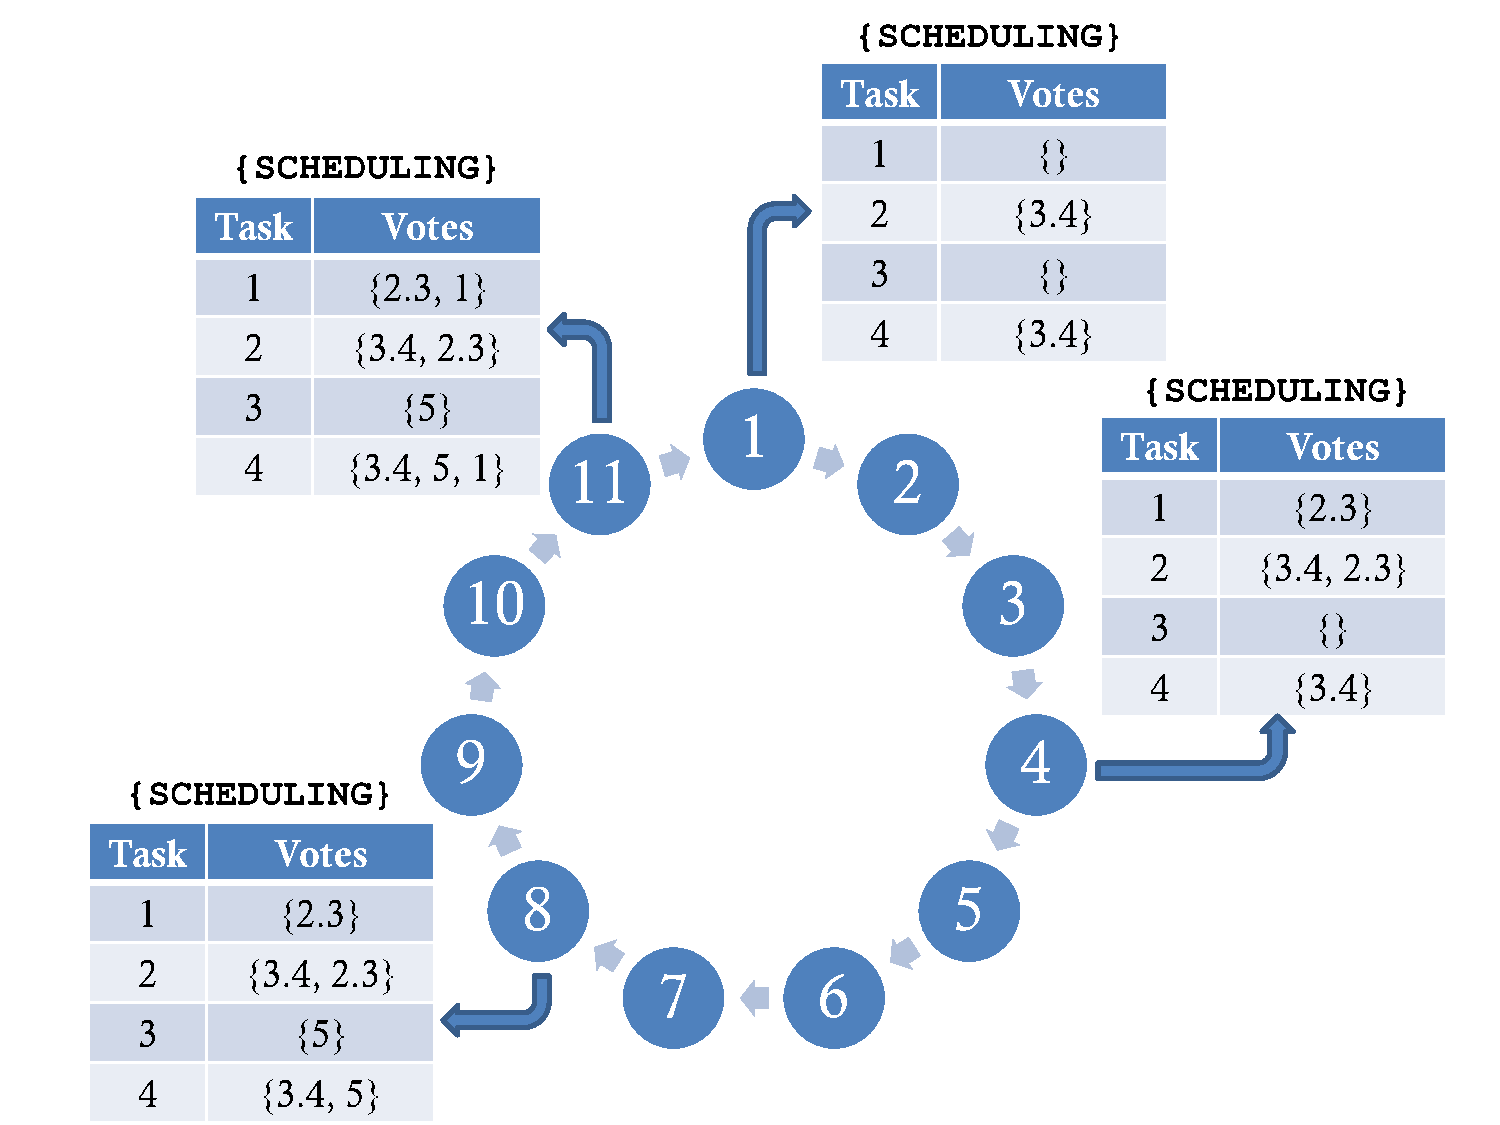
\includegraphics[width=\linewidth]{Figures/ring_1.pdf}
  \end{minipage}  
  \begin{minipage}[b]{0.5\linewidth}
    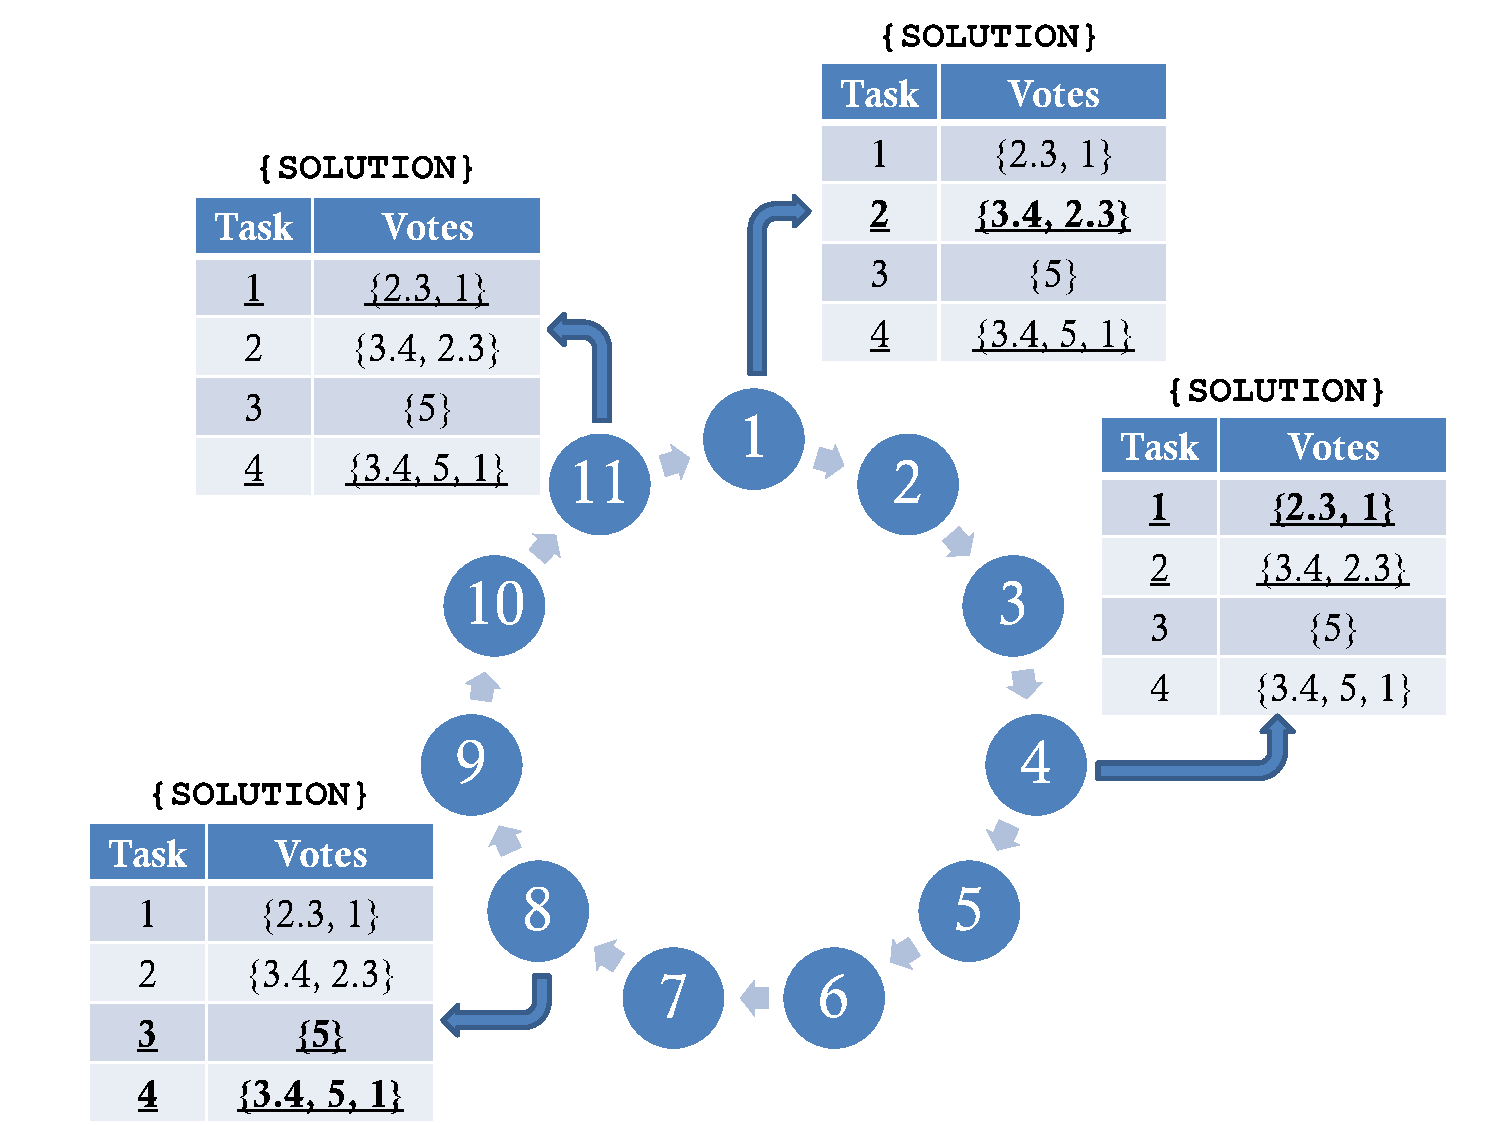
\includegraphics[width=\linewidth]{Figures/ring_2.pdf}
  \end{minipage}
  \caption{Ring-based scheduler approach}\label{fig_ring}
\end{figure}

It is assumed that the satellites in the system are physically\footnote{In fact, the ring formation is a practical architecture for satellite constellations.} or logically ordered, so that each satellite knows who its successor is and is able to communicate with it. When a task scheduling process is triggered, the global layer sends to a \emph{master} satellite the set of tasks to be performed. Then the master satellite runs its local scheduler to provide a number of local scheduling sub-solutions for them. Then, it builds up a message with the task set and votes the best sub-solution of those that he has found. The vote consists on \emph{marking} with the sub-solution's \emph{figure of merit} every single task scheduled in that particular sub-solution. This SCHEDULING message is sent to its successor in the ring. At each step, each satellite calculates a number of scheduling sub-solutions and votes the corresponding tasks.

Eventually, the message arrives again to the \emph{master} satellite --he will recognize this message as it will contain its own votes--. Now, the master changes the message type to SOLUTION and looks for the tasks that he had voted. He will effectively assign himself those tasks in which his vote is the highest one. The message travels around the ring again and when it turns to the \emph{master} leader, the scheduling process finishes. In Fig. \ref{fig_ring} a satellite ring formed by 11 nodes is scheduling a set of four tasks. Observe that not all the nodes vote for tasks, as they may not have resources for performing the tasks. In the SOLUTION phase, the previously voted tasks are underlined and bold text is used for tasks finally assigned to the satellite. 

Another variation would be that instead of having only one \emph{voting} round, there could be many of them. At each new round, if the satellite has not won the previous \emph{voting} round, it would vote the tasks of other calculated sub-solution. The algorithm converges to a consensual solution when no more sub-solutions can be voted or every satellite has won the previous \emph{voting} round for the tasks it voted.